% =========================================================================
% SciPost LaTeX template
% Version 1e (2017-10-31)
%
% Submissions to SciPost Journals should make use of this template.
%
% INSTRUCTIONS: simply look for the `TODO:' tokens and adapt your file.
%
% - please enable line numbers (package: lineno)
% - you should run LaTeX twice in order for the line numbers to appear
% =========================================================================


% TODO: uncomment ONE of the class declarations below
% If you are submitting a paper to SciPost Physics: uncomment next line
\documentclass[submission, Phys]{SciPost}
% If you are submitting a paper to SciPost Physics Lecture Notes: uncomment next line
%\documentclass[submission, LectureNotes]{SciPost}
% If you are submitting a paper to SciPost Physics Proceedings: uncomment next line
%\documentclass[submission, Proceedings]{SciPost}


\usepackage{graphicx}% Include figure files
\usepackage{subcaption}
\usepackage[labelformat=parens,labelsep=quad, skip=3pt]{caption}
\usepackage{dcolumn}% Align table columns on decimal point
\usepackage{bm}% bold math
\usepackage{xcolor}
\usepackage{hyperref}
\usepackage{afterpage}
\usepackage{bbold}
\usepackage{amssymb}
% below, packages for all kinds of unicode symbols
%\usepackage{amsmath}
%\usepackage{amsxtra}
%\usepackage{bbold}
%\usepackage{isomath}
%\usepackage{mathdots}
%\usepackage{stmaryrd}
\usepackage{wasysym}
%\usepackage{natbib}


% numerical scales
%\newcommand{\stiny}{\scalebox{0.5}{x}}
%\newcommand{\ssmall}{\scalebox{0.9}{x}}
%\newcommand{\smedium}{\scalebox{1.3}{x}}
%\newcommand{\slarge}{\scalebox{1.7}{x}}

%\newcommand{\stiny}{\scalebox{0.5}{s}}
%\newcommand{\ssmall}{\scalebox{0.9}{s}}
%\newcommand{\smedium}{\scalebox{1.3}{s}}
%\newcommand{\slarge}{\scalebox{1.7}{s}}

\newcommand{\stiny}{\scalebox{0.5}{s}}
\newcommand{\ssmall}{\scalebox{0.9}{s}}
\newcommand{\smedium}{\scalebox{1.3}{s}}
\newcommand{\slarge}{\scalebox{1.7}{s}}

%\newcommand{\stiny}{\scalebox{0.5}{\CIRCLE}}
%\newcommand{\ssmall}{\scalebox{0.9}{\CIRCLE}}
%\newcommand{\smedium}{\scalebox{1.3}{\CIRCLE}}
%\newcommand{\slarge}{\scalebox{1.7}{\CIRCLE}}

\newcommand{\U}{\left[
	\begin{array}{cccc}
		\ssmall & \ssmall & \ssmall & \ssmall \\
		\ssmall & \ssmall & \ssmall & \ssmall \\
		\ssmall & \ssmall & \ssmall & \ssmall \\
		\ssmall & \ssmall & \ssmall & \ssmall \\
	\end{array}
	\right]}

\newcommand{\Dp}{\left[
	\begin{array}{cccc}
		\slarge &  &  &  \\
		& \smedium &  &  \\
		&  & \ssmall &  \\
		&  &  & \ssmall \\
	\end{array}
	\right]}

\newcommand{\Dm}{\left[
	\begin{array}{cccc}
		\ssmall &  &  &  \\
		& \ssmall &  &  \\
		&  & \ssmall &  \\
		&  &  & \stiny \\
	\end{array}
	\right]}


\newcommand{\D}{\left[
	\begin{array}{cccc}
		\slarge &  &  &  \\
		& \smedium &  &  \\
		&  & \ssmall &  \\
		&  &  & \stiny \\
	\end{array}
	\right]}

\begin{document}

% TODO: write your article's title here.
% The article title is centered, Large boldface, and should fit in two lines
\begin{center}{\Large \textbf{
Fast and stable determinant quantum Monte Carlo in Julia
}}\end{center}

% TODO: write the author list here. Use initials + surname format.
% Separate subsequent authors by a comma, omit comma at the end of the list.
% Mark the corresponding author with a superscript *.
\begin{center}
Carsten Bauer\textsuperscript{1*}
\end{center}

% TODO: write all affiliations here.
% Format: institute, city, country
\begin{center}
{\bf 1} Institute for Theoretical Physics, University of Cologne, 50937 Cologne, Germany
\\
% TODO: provide email address of corresponding author
* bauer@thp.uni-koeln.de
\end{center}

\begin{center}
\today
\end{center}

% For convenience during refereeing: line numbers
%\linenumbers

\section*{Abstract}
{\bf
% TODO: write your abstract here.
In these notes we assess numerical stabilization methods employed in fermion many-body quantum Monte Carlo simulations. In particular, we empirically compare various matrix decomposition and inversion schemes to gain control over numerical instabilities arising in the computation of equal-time and time-displaced Green's functions within the determinant quantum Monte Carlo (DQMC) framework. Based on this comparison, we identify a procedure based on pivoted QR decompositions which is both accurate - to machine precision - and efficient. The Julia programming language is used for our assessment and we provide implementations of all discussed algorithms in the open-source software library \href{http://github.com/crstnbr/StableDQMC.jl}{\texttt{StableDQMC.jl}}.
}


% TODO: include a table of contents (optional)
% Guideline: if your paper is longer that 6 pages, include a TOC
% To remove the TOC, simply cut the following block
\vspace{10pt}
\noindent\rule{\textwidth}{1pt}
\tableofcontents\thispagestyle{fancy}
\noindent\rule{\textwidth}{1pt}
\vspace{10pt}





\section{Introduction}


Many-fermion systems play an important role in condensed matter physics. Due to their intrinsic correlations they feature rich phase diagrams which can not be captured by purely classical or non-interacting theories. Especially at the lowest temperatures, quantum mechanical fluctuations driven by Heisenberg's uncertainty principle become relevant and lead to novel states of matter like superconductivity or ones beyond the Fermi liquid paradigm. Because of the presence of interactions, predicting microscopic and thermodynamic properties of fermion many-body systems is inherently difficult. Analytical approaches are typically doomed to fail in cases where one can not rely on the smallness of an expansion parameter.

Fortunately, the determinant quantum Monte Carlo (DQMC) method overcomes this limitation. The key feature of DQMC is that it is numerically exact - given sufficient computation time the systematical error is arbitrarily small. Provided the absence of the famous sign-problem, it allows us to efficiently explore the relevant region of the exponentially large configuration space in polynomial time. It is an important unbiased technique for obtaining reliable insights into the physics of many-fermion systems.

Although conceptually straightforward, care has to be taken in implementing DQMC due to inherent numerical instabilities. It is the purpose of these notes to review stabilization schemes to heal those algebraic issues and to compare them with respect to accuracy and speed.
Specifically, the structure of this manuscript is as follows. We start by providing a brief introduction into the DQMC method in Sec.~\ref{sec:QMC}. In Sec.~\ref{sec:instabilities} we illustrate numerical instabilities arising in the DQMC formalism and discuss their origin. Following this, we present (Sec.~\ref{sec:stabilization}) and benchmark (Sec.~\ref{sec:benchmarks}) different numerical stabilization schemes in the context of the computation of the equal-times Green's function and its determinant. Lastly, we turn to the calculation of the time-displaced Green's function in Sec.~\ref{sec:TDGF} before concluding and summarizing in Sec.~\ref{sec:discussion}.

In the spirit of reproducible science, we provide implementations of all discussed algorithms, as well as the code to recreate all the plots of these notes, in form of the Julia package \href{http://github.com/crstnbr/StableDQMC.jl}{\texttt{StableDQMC.jl}}. This library is also intended to serve as an important abstraction layer: users can focus on the physical application rather than numerical instabilities. Readers are invited to open issues or pull requests at the repository to discuss the present or add new stabilization routines.

\section{Determinant Quantum Monte Carlo}\label{sec:QMC}

We begin by recalling the determinant quantum Monte Carlo (DQMC) algorithm \cite{Blankenbecler1981} for a generic quantum field theory that can be split into a purely bosonic part $S_B$ and a part $S_F$. The latter comprises fermion kinetics $T$ and boson-fermion interactions $V$. An example is the famous Hubbard model after decoupling the on-site
interaction $U n_{i, \uparrow} n_{i, \downarrow}$ by means of a Hubbard-Stratonovich or Hirsch transformation in either the spin or charge channel \cite{Hirsch1983}. As per usual, the central quantity of interest is the partition function
%
\begin{equation}
\mathcal{Z} = \int D\left( \psi, \psi^\dagger, \phi \right) e^{-S_B - S_F} \,.
\end{equation}
%
The basic idea of DQMC is to switch from the $d$ dimensional quantum theory to a $D = d + 1$ dimensional classical theory. The extra finite dimension of the classical theory is imaginary time $\tau$. It has a length proportional to the inverse temperature $\beta = 1/T$ and is discretized into $M$ time slices, $\beta = M \Delta \tau$. Applying a Trotter-Suzuki decomposition \cite{Trotter1959, Suzuki1986} one obtains
%
\begin{align}
	\mathcal{Z} &= \int D\phi \ e^{-S_B} \mathrm{Tr}{\left[\exp{\left( -\Delta\tau \sum_{l=1}^M \psi^\dagger \left[T + V_\phi\right] \psi \right)}\right]} \label{eq:discretizedpi} \,.
\end{align}
%
Next, the exponential is separated which leads to a systematic error of the order $\mathcal{O}\left(\Delta\tau^2\right)$,
\begin{align}
	e^{A + B} &\approx e^A e^B \quad \nonumber\\
	e^{-\Delta\tau (T + V)} &\approx e^{- \frac{\Delta\tau}{2}T} e^{-\Delta\tau V} e^{- \frac{\Delta\tau}{2}T} + \mathcal{O}\left(\Delta\tau^3\right), \nonumber\\
	\mathcal{Z} &= \int D\phi \ e^{-S_B} \mathrm{Tr}{\left[ \prod_{l=1}^{m} B_l \right]} + \mathcal{O}\left(\Delta\tau^2\right). \label{eq:Ztr}
\end{align}
%
Here, $B_l = e^{- \frac{\Delta\tau}{2}\psi^\dagger T \psi} e^{-\Delta\tau \psi^\dagger V_\phi \psi} e^{- \frac{\Delta\tau}{2}\psi^\dagger T \psi}$ are imaginary time slice propagators. Note that their potential contribution $e^{-\Delta\tau \psi^\dagger V_\phi \psi}$ depends on the boson $\phi$ due to fermion-boson coupling. Rewriting the trace in \eqref{eq:Ztr} as a determinant, an identity which can be proven \cite{Assaad2002a}, yields the fundamental form
%
\begin{align}
	\mathcal{Z} &= \int D\phi \ e^{-S_B} \det{G_\phi^{-1}} + \mathcal{O}\left(\Delta\tau^2\right), \label{eq:DQMC}
\end{align}
%
where
\begin{align}
	G = \left( \mathbb{1} + B_M B_{M-1} \cdots B_1 \right)^{-1} \label{etgf}
\end{align}
is the equal-time Green's function of the system.

According to Eq.~\eqref{eq:DQMC}, the probability weight appearing in a Metropolis Monte Carlo scheme reads
\begin{align}
	p = \min \left\{ 1 , e^{-\Delta S_\phi}  \dfrac{\det G}{\det G'} \right\}, \label{eq:metropolis}
\end{align}
which implies that, considering a generic update, one needs to compute the Green's function $G$ and it's determinant for both the current and the proposed state ($G'$) of the Markov walker. For local updates, however, one can typically avoid those costly calculations and rather compute the ratio of determinants in Eq.~\eqref{eq:metropolis} directly.

Importantly, it is only under specific circumstances, such as the presence of a symmetry, that the integral kernel can be safely interpreted as a probability weight as $G_\phi$ and its determinant are generally complex valued. This is the famous sign problem \cite{Li2019}.

\section{Numerical instabilities}\label{sec:instabilities}

To showcase the typical numerical instabilities arising in the DQMC framework we consider the Hubbard model in one dimension at half filling,
\begin{align}
	H = -t\sum_{\langle i,j \rangle} c_i^\dagger c_j + U \sum_i \left( n_{i\uparrow} - \frac{1}{2} \right) \left( n_{i\downarrow} - \frac{1}{2} \right) \label{eq:model},
\end{align}
and set the hopping amplitude to unity, $t=1$\footnote{We will consider the canonical discrete decoupling \cite{Hirsch1983} in the spin channel due to Hirsch.}.
%\begin{align}
%H = \left[
%\begin{array}{cccccccc}
%-0.1 & 1.0 &  &  &  &  &  &  \\
%1.0 & -0.1 & 1.0 &  &  &  &  &  \\
% & 1.0 & -0.1 & 1.0 &  &  &  &  \\
% &  & \ddots & \ddots & \ddots &  &  &  \\
%  &  &  & 1.0 & -0.1 & 1.0 &  \\
%  &  &  &  & 1.0 & -0.1 & 1.0 \\
%  &  &  &  &  & 1.0 & -0.1 \\
%\end{array}
%\right].
%\end{align}



As seen from Eq.~\eqref{etgf}, the building block of the equal-time Green's function is the slice matrix product chain
\begin{align}
	B(\beta, 0) \equiv B_M B_{M-1} \cdots B_1 = \underbrace{B B \cdots B}_{M \textrm{ factors}}. \label{eq:Bchain}
\end{align}
where in the second equality  we have assumed that the slice matrices are independent of imaginary time to simplify our numerical analysis\footnote{From a computational complexity point of view, this simplification is irrelevant. It corresponds to assuming a constant Hubbard-Stratonovich field.}.

First, we consider the non-interacting system, $U=0$. In Fig.~\ref{fig:naive_vs_stable}, we show that a naive computation of Eq.~\ref{eq:Bchain} is doomed to fail for $\beta \geq \beta_c \approx 10$. Leaving a discussion of the stabilization of the computation for the next section, let us highlight the origin of this instability. The eigenvalues of the system are given by
\begin{align}
	&\epsilon_k = -2t\cos(k).
\end{align}
The energy values are bounded by $-2t \leq \epsilon_k \leq 2t$. Hence, a single positive definite slice matrix $B = e^{-\Delta \tau T}$ has a condition number of about $\kappa \approx e^{4|t|\Delta \tau}$, which gives $\kappa \approx e^{4|t|M\Delta \tau} = e^{4|t|\beta}$ for  the product chain $B(\tau, 0)$. This implies that the scales present in $B(\tau, 0)$ broaden exponentially at low temperatures $T=1/\beta$ and roundoff errors due to finite machine precision will spoil a naive computation. We can estimate the inverse temperature of this breakdown of the calculation for the data type \texttt{Float64}, that is double floating-point precision according to the IEEE 754 standard \cite{Goldberg1991}, by solving $\kappa(\beta) \sim 10^{-17}$ for $\beta_c$. This gives $\beta_c \approx 10$ in good agreement with what we observe in Fig.~\ref{fig:naive_vs_stable}. Switching the data type to \texttt{Float128} (quadruple precision), we see in Fig.~\ref{fig:naive_vs_stable_float128} that the onset of roundoff errors is shifted to lower temperatures as expected.

Another consequence of these numerical imprecisions is that the $B(\tau, 0)$ obtained from a naive computation are generally not invertible such that the inversion in Eq.~\ref{etgf} is ill defined. This clearly prohibits a safe calculation of the equal-time Green's function and asks for more sophisticated techniques.


\begin{figure}
	\centering
	\begin{subfigure}{0.48\textwidth}
		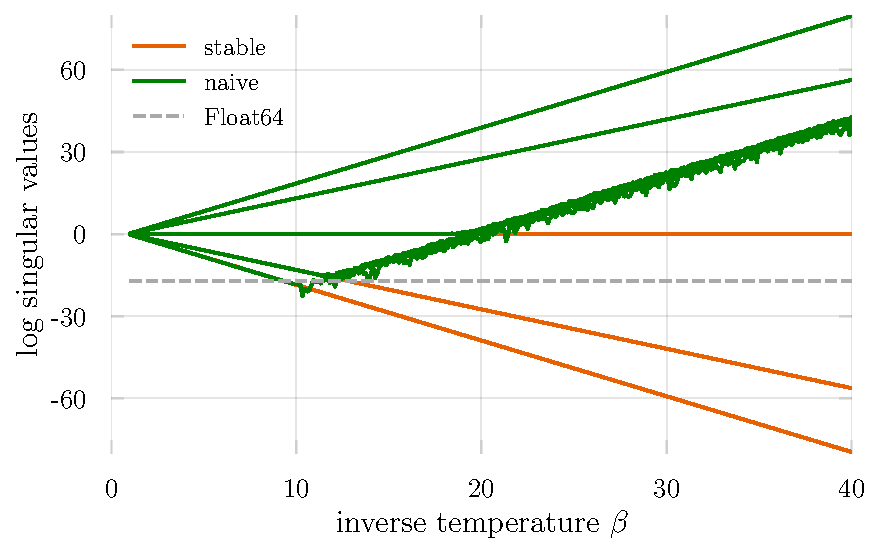
\includegraphics[width=\textwidth]{figures/naive_vs_stable.pdf}
		\caption{64-bit floating point (\texttt{Float64}) \label{fig:naive_vs_stable}}
	\end{subfigure}%
	\hspace{10pt}
	\begin{subfigure}{0.48\textwidth}
		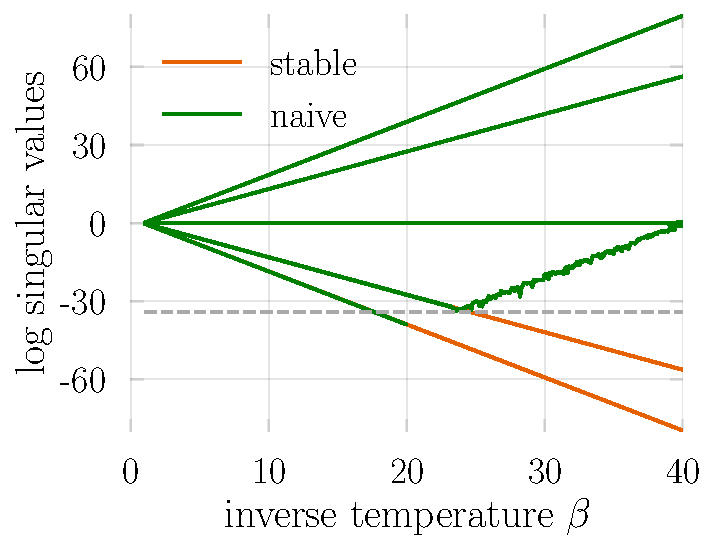
\includegraphics[width=\textwidth]{figures/naive_vs_stable_float128.pdf}
		\caption{128-bit floating point (\texttt{Float128}) \label{fig:naive_vs_stable_float128}}
	\end{subfigure}
	\vspace{5pt}
	\caption[MyCaption]{\textbf{Numerical instabilities} due to finite machine precision (green) arising in the calculation of the slice matrix product chain $B_M B_{M-1} \cdots B_1$ for model~\eqref{eq:model}. The dashed line (grey) indicates the expected floating point precision\protect\footnotemark. The arbitrary precision result (orange) is shown for comparison. Both considered binary floating point formats \texttt{Float64} (a) and \texttt{Float128} (b) are in compliance with the IEEE 754 standard.}
\end{figure}

\footnotetext{We estimate the precision as $p = \log_{10}(2^{\textrm{fraction}})$, where $\textrm{fraction}$ is the mantissa of a given binary floating point format. This gives $p\sim 16$ for \texttt{Float64} and $p\sim 34$ for \texttt{Float128}.}

\section{\label{sec:stabilization}Stabilization: matrix multiplications}

A trivial solution to the issue outlined above is to perform all numerical operations with arbitrary precision. In Julia this can be done by using the \texttt{BigFloat} data type\footnote{Technically, \texttt{BigFloat} has a finite, arbitrarily high precision.}. However, this comes at the expense of (unacceptable) slow performance due to algorithmic overhead and lack of hardware support. Arbitrary precision numerics is nevertheless a valuable tool and we will use it to benchmark the accuracy of stabilization methods below\footnote{For our non-interacting model system one can alternatively simply diagonalize the Hamiltonian and calculate the Green's function exactly.}.


How can we get a handle on the numerical instabilities in a floating point precision computation? The idea is to keep the broadly different scales separated throughout the computation (as much as possible) and only mix them in the final step, if necessary. A useful tool along these lines are matrix decompositions,
\begin{align}
	B = UDX. \label{eq:decomp}
\end{align}
Here, $U$ and $X$ are matrices containing scales of the order of unity and $D$ is a real diagonal matrix with the broad range of scales of $B$ separated on the diagonal. We will refer to the values in $D$ as singular values independent of the particular decomposition.

Instead of calculating products $B_2 B_1$ appearing in $B(\tau, 0)$, Eq.~\ref{eq:Bchain}, directly, we utilize Eq.~\ref{eq:decomp} to define a stable matrix multiplication (\texttt{fact\_mult} in \texttt{StableDQMC.jl})

\begin{align}
	B_2 B_1 &= \underbrace{U_2 D_2 X_2}_{B_2}\underbrace{U_1 D_1 X_1}_{B_1} \nonumber\\
	&= U_2 \underbrace{(D_2 ((X_2 U_1) D_1))}_{U' D' X'} X_1)\label{eq:stabmult}\\
	&= U_r D_r X_r. \nonumber
\end{align}
Here, $U_r = U_2 U'$, $D_r = D'$, $X_r = X' X_1$, and $U'D'X'$ indicates an intermediate matrix decomposition. If we follow this scheme, in which parentheses indicate the order of operations, largely different scales present in the diagonal matrices won't be mixed throughout the computation. Specifically, note that the multiplications of the well-conditioned, combined, unit-scale matrix $U = X_2 U_1$ with $D_1$ and $D_2$ do preserve the scale information: the diagonal matrices only rescale the columns and rows of the $U$,
\begin{align}
D_2  U D_1 &= \D  \U \D  \\
&= \D \left[
\begin{array}{cccc}
\ssmall\slarge & \ssmall\smedium & \ssmall^2 & \ssmall\stiny \\
\ssmall\slarge & \ssmall\smedium & \ssmall^2 & \ssmall\stiny \\
\ssmall\slarge & \ssmall\smedium & \ssmall^2 & \ssmall\stiny \\
\ssmall\slarge & \ssmall\smedium & \ssmall^2 & \ssmall\stiny \\
\end{array}
\right]\\
&= \left[
\begin{array}{cccc}
	\slarge^2\ssmall & \slarge\smedium\ssmall & \slarge\ssmall^2 & \slarge\ssmall\stiny \\
	\slarge\smedium\ssmall & \smedium^2\ssmall & \smedium\ssmall^2 & \smedium\ssmall\stiny \\
	\slarge\ssmall^2 & \smedium\ssmall^2 & \ssmall^3 & \ssmall^2\stiny \\
	\slarge\ssmall\stiny & \smedium\ssmall\stiny & \ssmall^2\stiny & \ssmall\stiny^2 \\
\end{array}
\right].
\end{align}

Repeating the procedure \eqref{eq:stabmult}, we obtain a numerically accurate $UDX$ decomposition of the full slice matrix product chain $B(\tau, 0)$.\footnote{Note that we do not discuss the option to calculate $B^M$ as $U D^M X$. This is intentional since most real systems will involve fermion-boson interactions and the slice matrices will depend on $\phi(\tau)$.} We note in passing that in a practical DQMC implementation it is often unnecessary to stabilize every single matrix product. Instead one typically performs a mixture of naive and stabilized products for the sake of speed while still retaining numerical accuracy \cite{Assaad2002a}.

\subsection{Matrix decompositions}

So far we haven't specified a concrete decomposition ${B = UDX}$. In fact, there are a couple of choices, two of which we will focus on in what follows.

\subsubsection{SVD ($UDV^\dagger$)}
A singular value decomposition (SVD) is given by
\begin{align}
	B = USV^\dagger,
\end{align}
where $U$ is unitary, $S$ is a real diagonal matrix, and $V^\dagger$ is unitary.

Julia offers a couple of purely-Julia SVD implementations, like \href{https://github.com/JuliaLinearAlgebra/GenericSVD.jl/}{GenericSVD.jl}, which we will use for \texttt{BigFloat} computations. However, some of the most optimized algorithms are part of LAPACK \cite{LAPACK} and Julia defaults to those algorithms for regular floating point types. Concretely, there are three SVD functions\footnote{Note that Fortran LAPACK functions are named according to realness and symmetries of the matrix. In Julia multiple-dispatch takes care of routing different matrix types to different \textit{methods}. The Julia function \texttt{gesdd} works for both real and complex matrices, i.e. there is no (need for) \texttt{cgesdd}.} implementing different algorithms for calculating the SVD:
\begin{itemize}
	\item \texttt{gesdd} (default): Divide-and-conquer (D\&C)
	\item \texttt{gesvd}: Conventional
	\item \texttt{gesvj}: Jacobi algorithm (through \href{https://github.com/RalphAS/JacobiSVD.jl}{JacobiSVD.jl})
\end{itemize}
which can be readily accessed via convenience wrappers of the same name exported by \texttt{StableDQMC.jl}. We will compare all of them below.

\subsubsection{QR ($UDT$)}
A QR decomposition reads
\begin{align}
	B = QR = UDT,
\end{align}
where we have split $R$ into a diagonal piece $D$ and upper triangular piece $T$. Hence, $U = Q$ is unitary, $D = \textrm{diag}(R)$ is a real diagonal matrix, and $T$ is upper triangular. In Julia, one can obtain the $QR$ factored form of a matrix by calling the function \texttt{qr} from the standard library \texttt{LinearAlgebra}\footnote{We use a pivoted QR in our analysis.}. Analogously, a decomposition into $UDT$ form is provided by \texttt{udt} and \texttt{udt!} in \texttt{StableDQMC.jl}.

\section{Stabilization: equal-time Green's function}

\subsection{Inversion schemes}
Looking at the equal-time Green's function in Eq.~\ref{etgf}, we have to be careful to keep scales separate as much as possible in adding the identity, which will wash out small singular values, and performing the inversion of $1 + B(\beta, 0)$.

A straightforward procedure (\texttt{inv\_one\_plus}) to add the unit matrix and perform the inversion in a stabilized manner is given by \cite{Santos2003, Assaad2002a}

\begin{align}
	G &= [\mathbb{1} + UDX]^{-1} \nonumber \\
	&= [U\underbrace{(U^\dagger X^{-1} + D)}_{udx}X]^{-1} \nonumber\\
	&= [(Uu)d(xX)]^{-1} \label{eq:inversion}\\
	&= U_r D_r X_r \nonumber,
\end{align}
with $U_r = (xX)^{-1}$, $D_r = d^{-1}$, $X_r = (Uu)^{-1}$. Here, the intermediate addition (parentheses in the second line of \eqref{eq:inversion}) of unit scales and singular values is separated from the unitary rotations,
\begin{align}
U^\dagger X^{-1} + D = \U + \D = \left[
\begin{array}{cccc}
\slarge & \ssmall & \ssmall & \ssmall \\
\ssmall & \smedium & \ssmall & \ssmall \\
\ssmall & \ssmall & \ssmall & \ssmall \\
\ssmall & \ssmall & \ssmall & \ssmall \\
\end{array}
\right].
\end{align}

However, when combined with certain matrix decompositions, this scheme will still fail to give accurate results for the equal-time Green's function $G$, as we will demonstrate below. Therefore we consider another stabilization scheme for the inversion \cite{Loh2005, Loh1989} (\texttt{inv\_one\_plus\_loh}), in which we initially separate the scales in $D$ as $D_p = \max(D, 1)$ and $D_m = \min(D, 1)$,
\begin{align}
D_p = \Dp, \quad D_m = \Dm,
\end{align}
and perform two intermediate decompositions,
\begin{align}
	G &= [\mathbb{1} + UDX]^{-1} \nonumber\\
	&= [\mathbb{1} + UD_mD_pX]^{-1} \nonumber\\
	&= [(X^{-1} D_p^{-1} + U D_m) D_p X]^{-1} \label{eq:inversion_loh} \\
	&= X^{-1} \underbrace{[D_p^{-1} (\underbrace{X^{-1} D_p^{-1} + UD_m}_{udx})^{-1}]}_{udx} \nonumber \\
	&= U_r D_r X_r, \nonumber
\end{align}
with $U_r = X^{-1}u$, $D_r = d$, and $X_r = x$.
\begin{align}
	X^{-1} D_p^{-1} + UD_m &\approx \left[
	\begin{array}{cccc}
	\ssmall + \ssmall/\slarge & \ssmall + \ssmall/\smedium & \ssmall& \ssmall\stiny + \ssmall \\
	\ssmall + \ssmall/\slarge & \ssmall + \ssmall/\smedium & \ssmall& \ssmall\stiny + \ssmall \\
	\ssmall + \ssmall/\slarge & \ssmall + \ssmall/\smedium & \ssmall& \ssmall\stiny + \ssmall \\
	\ssmall + \ssmall/\slarge & \ssmall + \ssmall/\smedium & \ssmall& \ssmall\stiny + \ssmall \\
	\end{array}
	\right] \approx \left[
	\begin{array}{cccc}
	\ssmall + \ssmall/\slarge & \ssmall + \ssmall\stiny & \ssmall& \ssmall\stiny + \ssmall \\
	\ssmall + \ssmall/\slarge & \ssmall + \ssmall\stiny & \ssmall& \ssmall\stiny + \ssmall \\
	\ssmall + \ssmall/\slarge & \ssmall + \ssmall\stiny & \ssmall& \ssmall\stiny + \ssmall \\
	\ssmall + \ssmall/\slarge & \ssmall + \ssmall\stiny & \ssmall& \ssmall\stiny + \ssmall \\
	\end{array}
	\right] \\
D_p^{-1} (udx)^{-1} &\approx \left[
\begin{array}{cccc}
\ssmall/\slarge & \ssmall/\slarge & \ssmall/\slarge & \ssmall/\slarge \\
\ssmall/\smedium & \ssmall/\smedium & \ssmall/\smedium & \ssmall/\smedium \\
\ssmall & \ssmall & \ssmall & \ssmall \\
\ssmall & \ssmall & \ssmall & \ssmall \\
\end{array}
\right].
\end{align}

\subsection{Benchmarks}\label{sec:benchmarks}

In the following we want to assess how the mentioned matrix decompositions perform in stabilized computations of $B(\beta, 0)$, the Green's function $G$, and its determinant $\det G$, both with respect to accuracy and speed. All results are for the Hubbard model, Eq.~\ref{eq:model}, with $U=0$ and $U=1$ (alpha transparent in all plots)

\subsubsection{Accuracy}

\begin{figure}
	\centering
	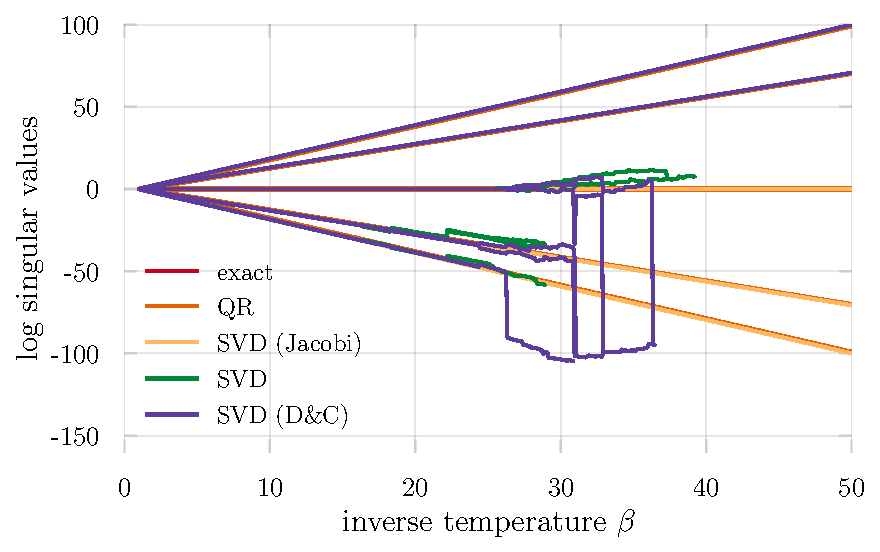
\includegraphics[width=0.8\textwidth]{figures/decomp_comparison_simple.pdf}
	\caption{\textbf{Comparison of matrix decompositions} to heal the numerical instabilities in the calculation of the slice matrix product chain $B_M B_{M-1} \cdots B_1$ for model~\eqref{eq:model}. The QR and Jacobi SVD singular values seem to lie on top of the exact ones whereas regular SVD and divide-and-conquer SVD show large deviations at low temperatures $\beta \gtrsim 25$ ($\Delta \tau = 0.1$).}
	\label{fig:decomp_comparison_simple}
\end{figure}

Before benchmarking the efficiency of an algorithm, it is crucial to check it's correctness first. Fig.~\ref{fig:decomp_comparison_simple} shows the log singular values of the slice matrix product chain $B(\beta, 0)$ stabilized with different matrix decompositions as a function of inverse temperature $\beta$. While QR and Jacobi SVD seem to lie on top of the numerically exact result, we observe large deviations for the simple and D\&C SVD algorithms at low temperatues ($\beta \gtrsim 25)$.\footnote{The fact that small scales are lost while large scales remain relatively accurate can be understood from LAPACK's SVD errorbounds \cite{errorbounds}.}\\


\begin{figure}
	\centering
	\begin{subfigure}{0.48\textwidth}
	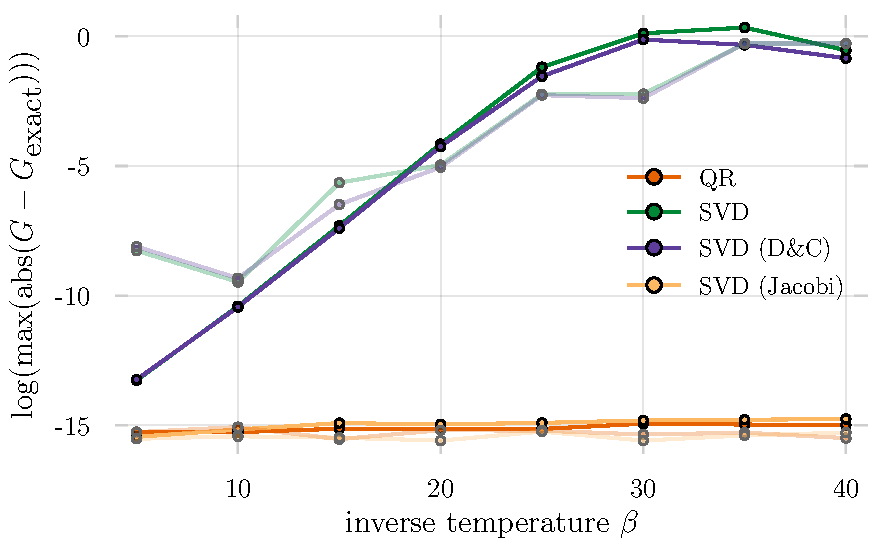
\includegraphics[width=\textwidth]{figures/accuracy_greens_svd_regularinv.pdf}
\caption{\texttt{inv\_one\_plus}, Eq.~\eqref{eq:inversion} \label{fig:greens_accuracy_regularinv}}
	\end{subfigure}%
	\hspace{10pt}
	\begin{subfigure}{0.48\textwidth}
	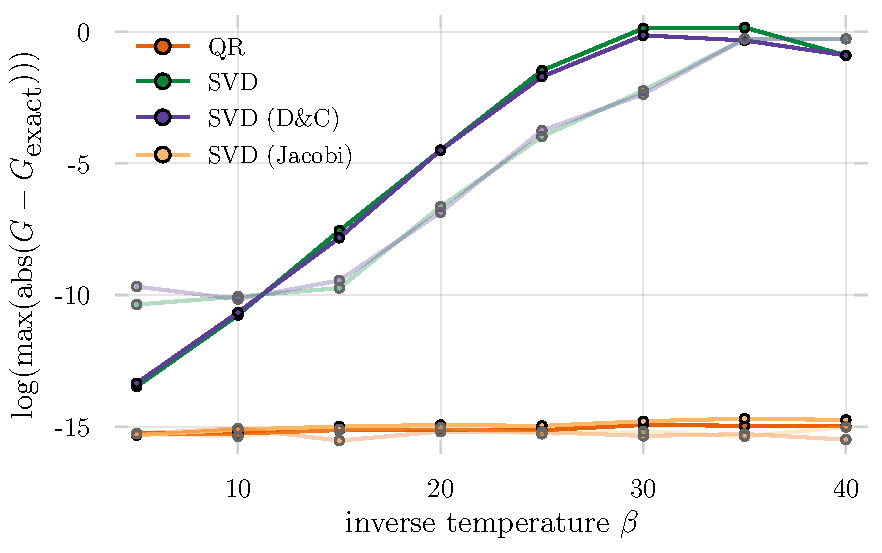
\includegraphics[width=\textwidth]{figures/accuracy_greens_svd_loh.pdf}
\caption{\texttt{inv\_one\_plus\_loh}, Eq.~\ref{eq:inversion_loh} \label{fig:greens_accuracy_loh}}
	\end{subfigure}
	\vspace{5pt}
	\caption{\textbf{Accuracy of the Green's function} obtained from stabilized computations using the listed matrix decompositions and the inversion schemes. Shown are results for $U=0$ (solid) and $U=1$ (alpha transparent).}
\end{figure}

Turning to the equal-time Green's function, Eq.~\ref{etgf}, we take the results for the slice matrix chains and perform the inversions according to the schemes presented above. We take the maximum absolute difference between the obtained Green's functions and the exact $G$ as an accuracy measure. The findings for the simple inversion scheme \texttt{inv\_one\_plus}, Eq.~\ref{eq:inversion}, are shown in Fig.~\ref{fig:greens_accuracy_regularinv}. At high temperatures and for $U=0$, all decompositions give the correct Green's function up to some limit close to floating point precision. However, at low temperatures only the QR decomposition and the Jacobi SVD reproduce $G_{\textrm{exact}}$ reliably. They have the highest accuracy by a large margin, followed by the other SVD variants, which  fail to reproduce the exact result accurately. As displayed in Fig.~\ref{fig:greens_accuracy_loh}, switching to the more careful procedure \texttt{inv\_one\_plus\_loh}, Eq.~\ref{eq:inversion_loh}, does generally improve the accuracy but the deviations seen for the regular and D\&C SVD schemes are still of order unity at low temperatures.


\begin{figure}
	\centering
	\begin{subfigure}{0.48\textwidth}
		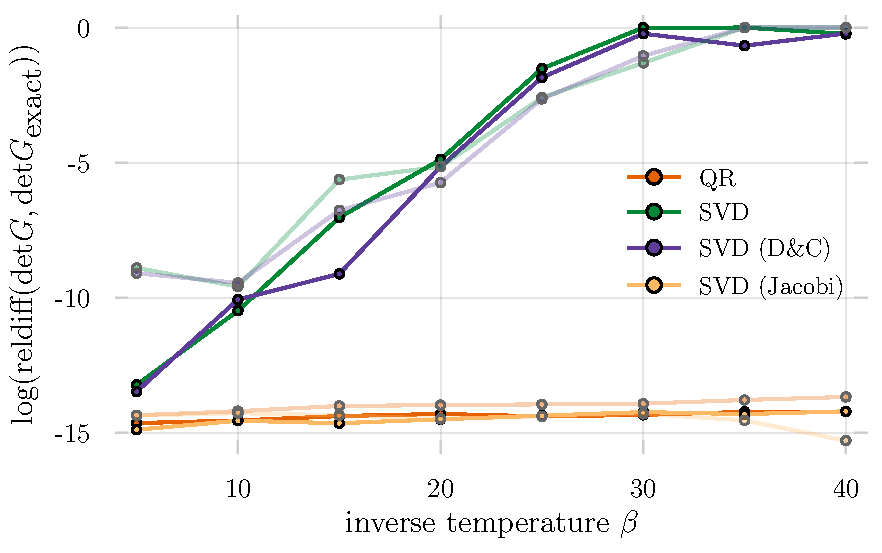
\includegraphics[width=\textwidth]{figures/accuracy_det_svd_regularinv.pdf}
		\caption{\texttt{inv\_one\_plus}, Eq.~\ref{eq:inversion}. \label{fig:det_accuracy_regularinv}}
	\end{subfigure}%
	\hspace{10pt}
	\begin{subfigure}{0.48\textwidth}
		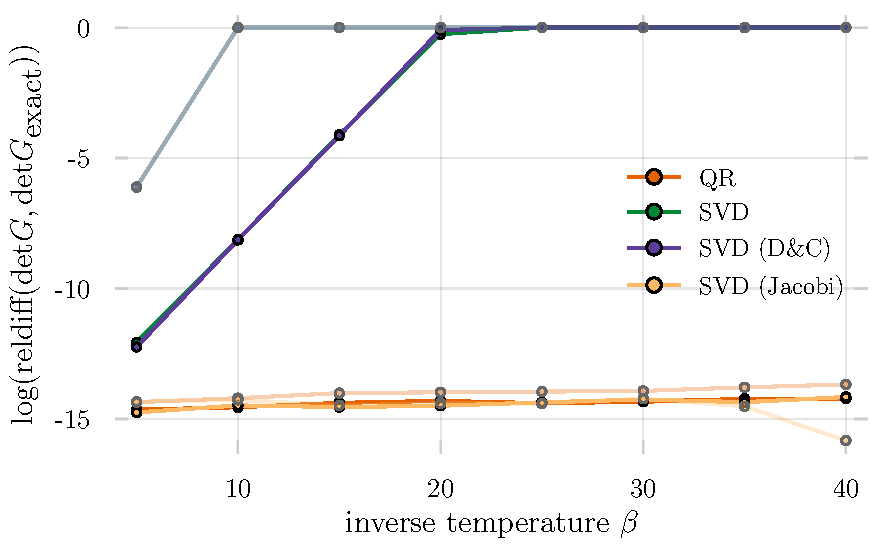
\includegraphics[width=\textwidth]{figures/accuracy_det_svd_loh.pdf}
		\caption{\texttt{inv\_one\_plus\_loh}, Eq.~\ref{eq:inversion_loh} \label{fig:det_accuracy_loh}}
	\end{subfigure}
	\vspace{5pt}
	\caption{\textbf{Accuracy of the determinant} of the equal-time Green's function obtained from stabilized computations using the listed matrix decompositions and the inversion schemes. Shown are results for $U=0$ (solid) and $U=1$ (alpha transparent).}
\end{figure}

In Figs.~\ref{fig:det_accuracy_regularinv},~\ref{fig:det_accuracy_loh} we show the logarithm of the relative error of the Green's function determinant, relevant in the Metropolis acceptance\footnote{For local updates on can generally avoid full calculations of Green's function determinants by exploiting locality and performing a Laplace expansion since only ratios of determinants appear in Eq.~\ref{eq:metropolis}. In fact, in an optimal implementation the computation of the acceptance rate is $O(1)$ rather than $O(N^3)$.}, obtained for all combinations of matrix decompositions and inversion schemes. Both the QR decomposition and the Jacobi SVD lead to accurate results for all accessed temperatures, irrespective of the employed inversion scheme. The other two SVD based methods on the other hand show large relative deviations for both \texttt{inv\_one\_plus} and \texttt{inv\_one\_plus\_loh}.

These findings suggest that only the QR decomposition and the Jacobi SVD are suited for computing both the equal time Green's function and it's determinant reliably, irrespective of the inversion procedure.

%\begin{table}[b]
%	\bgroup
%	\def\arraystretch{1.25}%  1 is the default, change whatever you need
%	\begin{tabular}{ccc}
%		$\beta = 5$ & Method & $\textrm{max}(\textrm{abs}(G - G_{\textrm{exact}}))$ \\
%		\hline
%		& QR & 6.1e-16 \\ 
%
%		& SVD, simple & 8.1e-14 \\ 
%
%		& SVD, D\&C & 6.9e-14 \\ 
%
%		& SVD, Jacobi & 6.1e-14 \\ 
%		\hline
%		& \\ 
%		$\beta = 40$ & Method & $\textrm{max}(\textrm{abs}(G - G_{\textrm{exact}}))$ \\
%		\hline
%		
%		& QR & 1.2e-15 \\ 
%
%		& SVD, simple & 4.7e-1 \\ 
%
%		& SVD, D\&C & 4.9e-1 \\ 
%
%		& SVD, Jacobi & 3.1e-4 \\ 
%		\hline
%	\end{tabular}
%	\egroup
%	\caption{\textbf{Accuracy of the Green's function} obtained from stabilized computations using the listed matrix decompositions at high ($\beta = 5$) and low temperatures ($\beta = 40$). \label{tbl:greens_accuracy}}
%\end{table}




%\begin{table}
%	\bgroup
%	\def\arraystretch{1.25}%  1 is the default, change whatever you need
%	\begin{tabular}{cccc}
%		$\beta = 5$ & Method & $\Delta_\textrm{abs} (\textrm{det} G)$ & $\Delta_\textrm{rel}(\textrm{det} G)$ \\
%		\hline
%		& QR & 2.3e-27 & 1.1e-15 \\ 
%		
%		& SVD, simple & 3.2e-26 & 1.5e-14 \\ 
%		
%		& SVD, D\&C & 1.8e-25 & 8.5e-14 \\ 
%		
%		& SVD, Jacobi & 1.2e-25 & 5.7e-14 \\ 
%		\hline
%		& \\ 
%		$\beta = 40$ & Method & $\Delta_\textrm{abs}(\textrm{det} G)$ & $\Delta_\textrm{rel}(\textrm{det} G)$ \\
%		\hline
%		
%		& QR & 4.1e-107 & 7.7-15 \\ 
%		
%		& SVD, simple & 4.5e-90 & 1.0e-0 \\ 
%		
%		& SVD, D\&C & 2.6e-93 & 1.0e-0 \\ 
%		
%		& SVD, Jacobi & 8.8e-97 & 1.7e-4 \\ 
%		\hline
%	\end{tabular}
%	\egroup
%	\caption{\textbf{Accuracy of the determinant} of the equal-time Green's function obtained from stabilized computations using the listed matrix decompositions at high ($\beta = 5$) and low temperatures ($\beta = 40$). \label{tbl:det_accuracy}}
%\end{table}



\subsubsection{Efficiency}

Independent of the deployed inversion scheme, matrix decompositions account for most of the computational cost in the Green's function calculation. Fig.~\ref{fig:benchmark_decomps} illustrates the raw efficiency of all SVDs relative to the QR decomposition. While the conventional SVD and the Jacobi SVD are about an order of magnitude slower, the divide-and-conquer based SVD is in the same ballpark as the QR decomposition. The Jacobi SVD variant is, by far, the most costly of all considered matrix decompositions, being 10 times more time consuming than the QR decomposition, even for small system sizes.

Since the decompositions represent the performance bottleneck, we expect that these speed differences propagate and dominate benchmarks of the full Green's function computations. As visible in Figs.~\ref{fig:greens_accuracy_regularinv} and \ref{fig:greens_accuracy_loh}, this anticipation is qualitatively confirmed up to numerical deviations. Independent of the deployed inversion scheme, the divide-and-conquer SVD can compete with the QR decomposition in terms of speed whereas the other SVD algorithms unambiguously fall behind. We note that the relative slowdown factor is larger for the scheme by Loh \textit{et al.}, which is understood from the fact that it requires two intermediate matrix decompositions rather than one.

\begin{figure}
	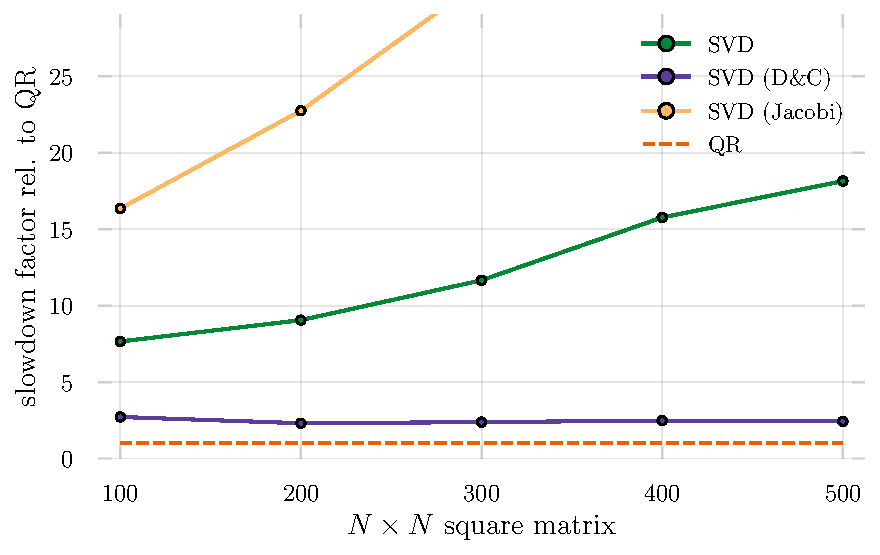
\includegraphics[width=0.8\textwidth]{figures/benchmark_decomps.pdf}
	\caption{\textbf{Efficiency of different matrix decompositions}. Shown are the slowdown factors of single SVDs relative to a QR decomposition of a complex matrix of size $N \times N$. \label{fig:benchmark_decomps}}
\end{figure}


\begin{figure}
	\centering
	\begin{subfigure}{0.48\textwidth}
			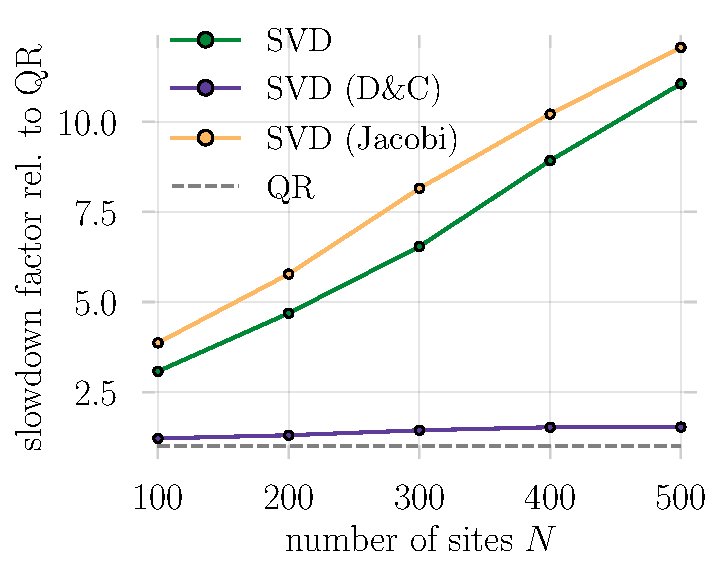
\includegraphics[width=\textwidth]{figures/benchmark_fact_inv_one_plus.pdf}
		\caption{\texttt{inv\_one\_plus}, Eq.~\eqref{eq:inversion}. \label{fig:greens_benchmark_regularinv}}
	\end{subfigure}%
	\hspace{10pt}
	\begin{subfigure}{0.48\textwidth}
		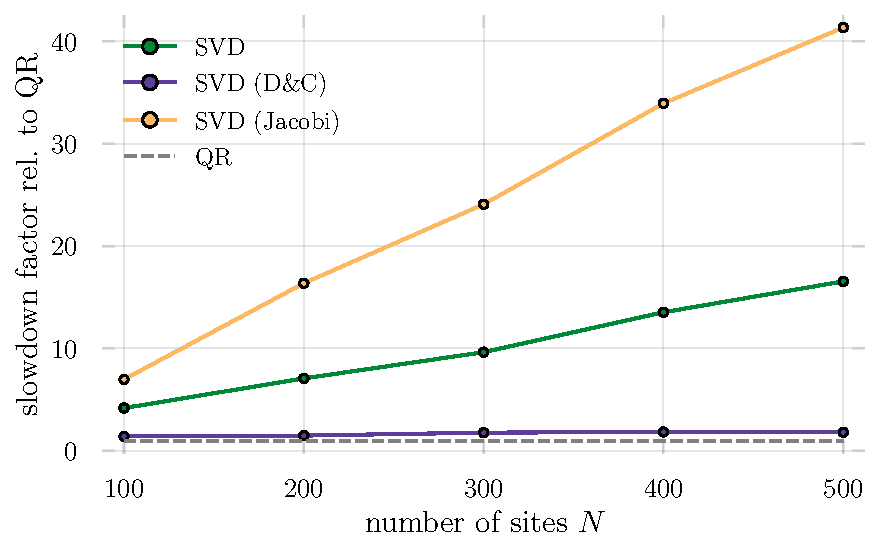
\includegraphics[width=\textwidth]{figures/benchmark_fact_inv_one_plus_loh.pdf}
		\caption{\texttt{inv\_one\_plus\_loh}, Eq.~\eqref{eq:inversion_loh}. \label{fig:greens_benchmark_loh}}
	\end{subfigure}
	\vspace{5pt}
	\caption{\textbf{Efficiency of the stabilized Green's function calculation} using the listed matrix decompositions and the inversion schemes. Shown are results for $U=0$.}
\end{figure}


%\afterpage{\clearpage}
\section{Stabilization: time-displaced Green's function}\label{sec:TDGF}

\textcolor{red}{TODO: Motivate TDGF. Why interesting? It is not need in the plain DQMC.}

We generalize our definition of the equal times Green's function, Eq.~\ref{etgf}, to include the imaginary time $\tau = l \Delta \tau$ dependence,
\begin{align}
	G(\tau) = \langle c_{i} c_{j}^\dagger \rangle_{\phi_l} = \left( 1 + B_{l-1}\dots B_1 B_M \dots B_l \right)^{-1}.
\end{align}
Note that $ G \equiv G_1 = G_{M+1} = \left( 1 + B_M \dots B_l \right)^{-1} $. The time displaced Green's function can now be defined as \cite{Santos2003, Assaad2002a}
\begin{align*}
	G_{l_1,l_2} &\equiv G(\tau_1, \tau_2) \equiv \langle T c_i(\tau_1) c_j^\dagger(\tau_2) \rangle_\varphi,
\end{align*}
where $T$ represents time ordering.

More explicitly this reads
\begin{align}
	G(\tau_1, \tau_2) = \begin{cases}
		B_{l_1} \cdots B_{l_2 + 1} G_{l_2 + 1}, &\tau_1 > \tau_2,\\
		- \left( 1 - G_{l_1 + 1} \right) \left( B_{l_2} \cdots B_{l_1 + 1}\right)^{-1}, &\tau_2 > \tau_1.
	\end{cases} \label{eq:tdgf_propagate}
\end{align}
In principle, this gives us a prescription for how to calculate $G(\tau_1, \tau_2)$ from the equal time Green's function $G(\tau)$ (which we know how to stabilize). However, when $|\tau_1 - \tau_2|$ is large a naive calculation of slice matrix product chains in Eq.~\ref{eq:tdgf_propagate} would be numerically unstable, as seen above. Also, by first calculating $G$ we already mix important scale information in the last recombination step, in which we multiply $G = UDX$. We therefore rather compute the time-displaced Green's function directly as
\begin{align}
	G(\tau_1, \tau_2) = (U_L D_L X_L + U_R D_R X_R)^{-1}.
\end{align}

\subsection{Inversion schemes}
Similar to Sec.~\ref{sec:stabilization}, we must be very careful to keep the involved scales separated as much as possible when performing the summation and the inversion.
As a first explicit procedure, we consider a simple generalization of Eq.~\ref{eq:inversion} (\texttt{inv\_sum}),
\begin{align}
	G(\tau_1, \tau_2) &= [U_L D_L X_L + U_R D_R X_R]^{-1} \nonumber\\
	&= [U_L \underbrace{(D_L X_L X_R^{-1} + U_L^\dagger U_R D_R)}_{udx} X_R ]^{-1} \nonumber\\
	&= [(U_L u) d^{-1} (x X_R)]^{-1} \label{eq:inversion_tdgf}\\
	&= U_r D_r X_r, \nonumber 
\end{align}
where $U_r = (x X_R)^{-1}$, $D_r = d^{-1}$, and $X_r = (U_L u)^{-1}$.

A different scheme, analogous to Eq.~\ref{eq:inversion_loh}, where we split the scales in $D$, is as follows (\texttt{inv\_sum\_loh}), \cite{Loh2005}
\begin{align}
	G(\tau_1, \tau_2) &= [U_L D_L X_L + U_R D_R X_R]^{-1} \nonumber\\
	&= [U_L D_{Lm} D_{Lp} X_L + U_R D_{Rm} D_{Rp} X_R]^{-1} \nonumber\\
	&= \left[U_L D_{Lp} \underbrace{\left( \dfrac{D_{Lm}}{D_{Rp}} X_L X_R^{-1} + U_L^\dagger U_R \dfrac{D_{Rm}}{D_{Lp}} \right)}_{udx} X_R D_{Rp} \right]^{-1} \nonumber\\
	&= X_R^{-1} \underbrace{\dfrac{1}{D_{Rp}} [udx]^{-1} \dfrac{1}{D_{Lp}}}_{udx} U_L^\dagger \label{eq:inversion_tdgf_loh} \\
	&= U_r D_r X_r, \nonumber
\end{align}
with $U_r = X_R^{-1} u$, $D_r = d$, and $X_r = x U_L^\dagger$.

We note in passing that \cite{Hirsch1988} has proposed an alternative method for computing the time-displaced Green's function based on a space-time matrix formulation of the problem. Although this technique has been successfully deployed in many-fermion simulations we won't discuss it here because of its subpar computational scaling: for a system composed of $N$ lattice sites, fermion flavors $f$, and imaginary time extent $M$ one has to invert (naively a $\mathcal{O}(x^3)$ operation) a matrix which takes up $\mathcal{O}((NMf)^2)$ memory.

\begin{figure}[b]
	\centering
	\begin{subfigure}{0.48\textwidth}
		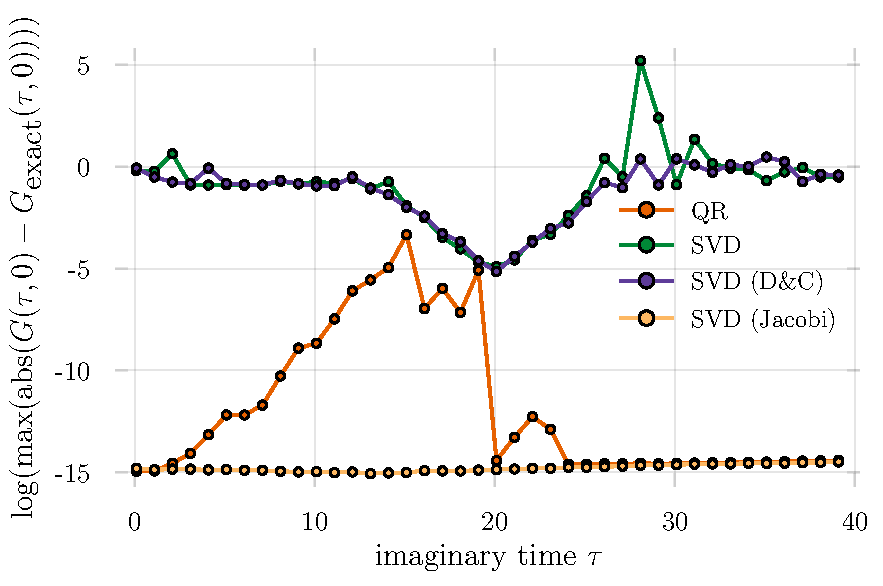
\includegraphics[width=\textwidth]{figures/accuracy_tdgf_U0.pdf}
		\caption{\texttt{inv\_sum}, Eq.~\eqref{eq:inversion_tdgf}. \label{fig:tdgf_accuracy_regularinv}}
	\end{subfigure}%
	\hspace{10pt}
	\begin{subfigure}{0.48\textwidth}
		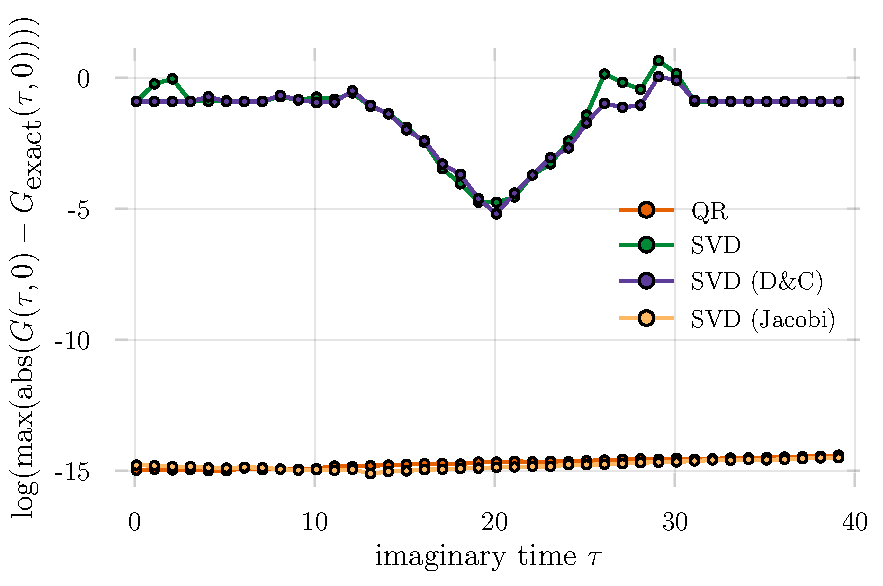
\includegraphics[width=\textwidth]{figures/accuracy_tdgf_loh_U0.pdf}
		\caption{\texttt{inv\_sum\_loh}, Eq.~\eqref{eq:inversion_tdgf_loh}. \label{fig:tdgf_accuracy_loh}}
	\end{subfigure}
	\vspace{5pt}
	\caption{\textbf{Accuracy of the time-displaced Green's function} obtained from stabilized computations using the listed matrix decompositions and the inversion schemes for $\beta = 40$.}
\end{figure}

\subsection{Benchmarks}
\subsubsection{Accuracy}

In Fig.~\ref{fig:tdgf_accuracy_regularinv}, we show the logarithmic maximal deviation of the time-displaced Green's function as calculated using the regular inversion scheme \texttt{inv\_sum} from the exact Green's function as a function of the time-displacement $\tau$ at inverse temperature $\beta=40$. Clearly, both non-Jacobi SVDs fail to capture the intrinsic scales sufficiently and errors much beyond floating point precision are seen. Although the QR decomposition systematically leads to equally or more accurate values for all considered imaginary times, it fails to be reliable at long times $\tau\sim\beta/2$ (recall that the Green's function is anti-periodic in $\tau$). Only the Jacobi SVD delivers reliable results for all considered imaginary times.

When switching to the inversion scheme \texttt{inv\_sum\_loh}, the situation changes, as can be seen in Fig.~\ref{fig:tdgf_accuracy_loh}. While the non-Jacobi SVDs show similar (insufficient) accuracy as when deployed in combination with \texttt{inv\_sum}, using the QR decomposition leads to stable Green's function estimates up to floating point precision across the entire imaginary time axis. Similar to our findings for the equal-time Green's function, this suggests that only the Jacobi SVD and the QR decomposition, when paired with the appropriate inversion procedure, are reliable in a DQMC context.

\subsubsection{Efficiency}\label{sec:tdgfbenchmark}

Finally, we compare the computational efficiency of the Jacobi SVD combined with the regular inversion and the QR decomposition paired with \texttt{inv\_sum\_loh}. As shown in Fig.~\ref{fig:tdgf_benchmark}, we find that the latter is consistently faster for all considered system sizes. In relative terms, the SVD based approach is at least a factor of two slower and seems to display inferior scaling with the chain length $N$. This indicates that in a DQMC context numerical stabilization via QR decompositions should be preferred despite the higher complexity of the inversion scheme.

\begin{figure}[t]
	\centering
	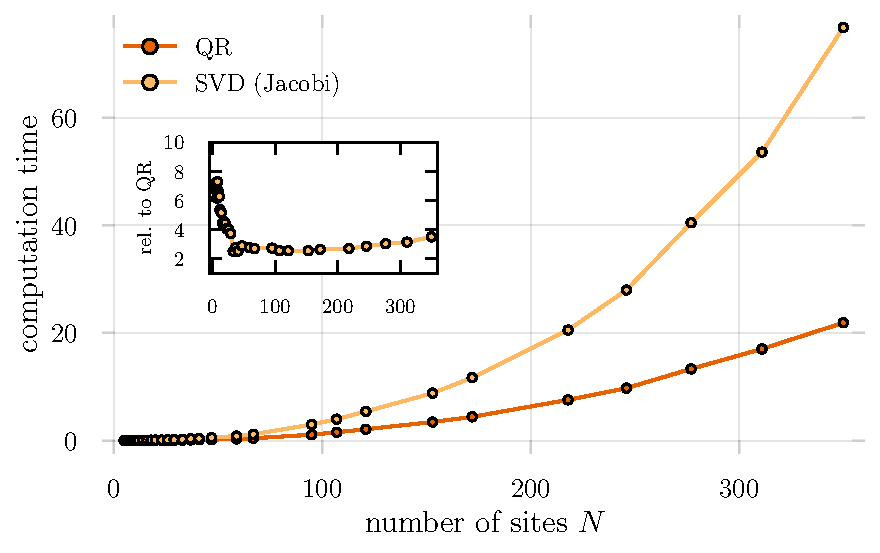
\includegraphics[width=0.8\textwidth]{figures/benchmark_jacobi_vs_qr_tdgf.pdf}
	\caption{\textbf{Efficiency of the time-displaced Green's function} obtained from stabilized computations using the QR decomposition in combination with the inversion scheme \texttt{inv\_sum\_loh}, Eq.~\eqref{eq:inversion_tdgf_loh} and the Jacobi SVD paired up with the regular inversion scheme \texttt{inv\_sum}, Eq.~\eqref{eq:inversion_tdgf}. Measurements are taken over multiple runs at $\tau = \beta/2 = 20$. The inset show the slowdown of the Jacobi SVD relative to the QR based approach. \label{fig:tdgf_benchmark}}
\end{figure}

\section{Discussion}\label{sec:discussion}

Numerical instabilities are naturally present in quantum Monte Carlo simulations of many-fermion systems. Different algorithmic schemes and matrix decomposition techniques have been proposed over time to handle the exponential spread of scales in a stable manner. However, as we have shown in these notes, they can have vastly different accuracy and efficiency rendering them more or less suited for determinant quantum Monte Carlo simulations.

For the considered one-dimensional Hubbard model, we were able to compute the equal-time Green's function and its determinant to floating point precision using the QR-based UDT decomposition and the Jacobi SVD. In case of the time-displaced Green's function, the QR had to be combined with the inversion algorithm suggested by ~\cite{Loh1989} while the Jacobi SVD was accurate irrespective of the inversion scheme. Conventional and divide-and-conquer based SVDs consistently failed to produce reliable results in both cases, in particular at the lowest considered temperatures, $\beta \sim 40$.

In terms of speed, we find that the QR decomposition outperforms the conventional and Jacobi SVDs by a large margin while only the D\&C SVD variant has similar computational efficiency. Since the inversion scheme in the QR case involves matrix divisions this observed performance difference is not exclusively due to - but dominated by - the computational cheapness of a QR decomposition compared to a SVD.

In summary, our assessment suggests that the QR decomposition is the best choice for DQMC simulations as it is both fast and stable. However, when utilized in the computation of time-displaced Green's functions, the accuray strongly depends on the chosen inversion scheme. Among the ones considered in these notes, only the algorithm by  ~\cite{Loh1989} could produce reliable results. The Jacobi SVD, although computationally more expensive, proved to be a stable alternative. We note that interested readers may find a more analytical comparison of the performance of QR and Jacobi SVD for DQMC in Ref.~\cite{Bai2011}.

Finally, let us remark that the performance of all stabilization schemes is affected by the condition number of the time slice matrices and is therefore model (parameter) dependent. While we have not investigated this dependence in systematic detail,  we nonetheless think that our major conclusions bear some universality and will hopefully serve as a useful guide.



\section*{Acknowledgements}
We thank Peter Bröcker, Yoni Schattner, Snir Gazit, and Simon Trebst for useful discussions and Frederick Freyer for identifying a few typos in this manuscript.

\paragraph{Funding information}
Mention CRC 183 funding here?


\begin{appendix}

\section{Inversion schemes for a slice matrix function stack}

In practical implementations of DQMC one typically stores intermediate decomposed slice matrix products $B(\tau_1, \tau_2)$ in a stack for reuse in future Green's function calculations \cite{Assaad2002a, Santos2003, Broecker2016}. In this case, the inversion procedure in Eq.~\eqref{eq:inversion} needs to be supplemented by a scheme to combine two elements $U_L, D_L, X_L$ and $U_R, D_R, X_R$ from the stack. Below we describe the latter for both matrix decompositions considered in the main text\footnote{In \texttt{StableDQMC.jl}, Julia's multiple dispatch will automatically select the correct method based on the number of provided UDT factorizations.}.

\subsection{QR/UDT}

(\texttt{StableDQMC.jl}: \texttt{inv\_one\_plus(::UDT, ::UDT)})
\begin{align}
	G &= \left[\mathbb{1} + U_L D_L T_L \left( U_R D_R T_R \right)^\dagger \right]^{-1}\nonumber \\
	&= \left[\mathbb{1} + U_L \underbrace{\left( D_L \left( T_L T_R^\dagger \right) D_R \right)}_{udt} U_R^\dagger \right]^{-1} \\
	&= \left[\mathbb{1} + U D T \right]^{-1},\nonumber
\end{align}
with $U=U_Lu$, $D=d$, and $T=tU_R^\dagger$. This $UDT$ factorization may now be substituted into Eq.~\eqref{eq:inversion}.


\subsection{SVD}

(\texttt{StableDQMC.jl}: \texttt{inv\_one\_plus(::SVD, ::SVD)})
\begin{align}
G &= \left[\mathbb{1} + U_L D_L V_L^\dagger U_R D_R V_R^\dagger \right]^{-1} \nonumber \\
&= \left[\mathbb{1} + U_L \underbrace{\left( D_L \left( V_L^\dagger U_R \right) D_R \right)}_{udv^\dagger} V_R^\dagger \right]^{-1} \\
&= \left[\mathbb{1} + U D V^\dagger \right]^{-1},\nonumber
\end{align}
with $U=U_Lu$, $D=d$, and $V=v V_R$. This SVD factorization may now be substituted into Eq.~\eqref{eq:inversion}.

	
\end{appendix}

%\section{About references}
%Your references should start with the comma-separated author list (initials + last name), the publication title in italics, the journal reference with volume in bold, start page number, publication year in parenthesis, completed by the DOI link (linking must be implemented before publication). If using BiBTeX, please use the style files provided  on \url{https://scipost.org/submissions/author_guidelines}.
%in order to simplify the production of your paper.


% TODO:
% Provide your bibliography here. You have two options:

% FIRST OPTION - write your entries here directly, following the example below, including Author(s), Title, Journal Ref. with year in parentheses at the end, followed by the DOI number.
%\begin{thebibliography}{99}
%\bibitem{1931_Bethe_ZP_71} H. A. Bethe, {\it Zur Theorie der Metalle. i. Eigenwerte und Eigenfunktionen der linearen Atomkette}, Zeit. f{\"u}r Phys. {\bf 71}, 205 (1931), \doi{10.1007\%2FBF01341708}.
%\bibitem{arXiv:1108.2700} P. Ginsparg, {\it It was twenty years ago today... }, \url{http://arxiv.org/abs/1108.2700}.
%\end{thebibliography}

% SECOND OPTION:
% Use your bibtex library
% \bibliographystyle{SciPost_bibstyle} % Include this style file here only if you are not using our template
\bibliography{references}

\nolinenumbers

\end{document}
